Los anemómetros son instrumentos capaces de medir el viento, miden la intensidad y la dirección respecto el norte geográfico. La medición del viento es crucial en una variedad de aplicaciones, tales como estudios de contaminación atmosférica, vigilancia y predicción meteorológica, aterrizaje de aeronaves, análisis climático en función de la carga de viento, evaluación de daños causados por el viento, estimación del potencial de energía eólica y aplicaciones agrarias. Como todo instrumento de medición, deben ser calibrados para asegurar la trazabilidad metrológica de las mediciones respecto a patrones estándar nacionales o internacionales \cite{wmoChapter8}. Tradicionalmente, los túneles de viento utilizados para tales calibraciones se operan de forma manual o semi-automática. En este trabajo, se automatizó el proceso de medición mediante el control del motor del túnel de viento con un controlador PID. Este controlador recibe referencias de velocidad del viento proporcionadas por un anemómetro patrón. Además, estas mediciones se utilizan para llevar a cabo el proceso de calibración de otros anemómetros que también son afectados por el mismo flujo de viento. En resumen, el sistema no solo controla las condiciones del viento de manera precisa, sino que también permite la calibración de instrumentos bajo calibración (IBC).

\section{Estado del arte}\label{sec:estado_del_arte}
A lo largo de los años, la tecnología de sensores de viento y los métodos de calibración han experimentado una evolución significativa, impulsada por la necesidad de mayor precisión y confiabilidad en las mediciones. En sus inicios, los anemómetros eran dispositivos mecánicos simples. Uno de los ejemplos más antiguos y utilizados es el anemómetro de copa, inventado por Thomas Romney Robinson en 1846. Este dispositivo consiste en tres o cuatro copas montadas en los extremos de brazos horizontales que giran alrededor de un eje vertical. La velocidad de rotación es proporcional a la velocidad del viento \cite{robinson1846}. La calibración de estos anemómetros se realizaba mediante métodos empíricos en campo abierto. Otro tipo histórico de anemómetro es el de hélice, que opera de manera similar al de copa pero utiliza una hélice en lugar de copas. Este diseño es especialmente útil para medir la velocidad del viento en una dirección específica \cite{robinson1846}. En la actualidad, la tecnología ha avanzado hacia anemómetros más sofisticados y precisos. Por ejemplo, los anemómetros de copas y veleta han incorporado electrónica y sensores internos a su sistema mecánico. Otro ejemplo, son los anemómetros sónicos que utilizan ondas ultrasónicas para medir la velocidad y dirección del viento, determinando el tiempo que tardan las ondas sonoras en viajar entre transductores. Estos anemómetros son altamente precisos y, al no tener partes móviles, requieren menos mantenimiento \cite{sonic_anemometers}. En el siguiente capitulo se darán mas detalles sobre éstos y otros tipos de anemómetros actuales. La calibración de los anemómetros en la actualidad se realiza en túneles de viento, instalando el anemómetro en la cámara de ensayos del túnel. El anemómetro se somete a un flujo de aire generado por el túnel, cuya velocidad se ajusta dentro de un rango específico. Durante el proceso, se compara la lectura del anemómetro con la de un instrumento patrón, asegurando que las mediciones sean precisas y trazables al Sistema Internacional (SI). La incorporación de electrónica digital con microcontroladores y su programación, junto con una aplicación web desarrollada con un \textit{framework} actual, ha permitido obtener un sistema completo e integral que garantiza la repetibilidad del proceso de calibración y la correcta documentación en una base de datos que ofrece numerosas ventajas para un laboratorio, incluyendo la capacidad de almacenar grandes volúmenes de datos de manera organizada, facilitando el acceso rápido y eficiente a la información, mejorando la gestión de datos y permitiendo un seguimiento preciso de los experimentos y calibraciones. Además, aseguran la integridad y seguridad de los datos, protegiéndolos contra pérdidas y accesos no autorizados.

\section{Motivación}\label{sec:motivacion}

El Servicio Meteorológico Nacional (SMN) representa al Centro Regional de Instrumentos de Buenos Aires (RIC III) de la Asociación Regional III \cite{RIC_Argentina}. Este Centro, dependiente de la Organización Mundial de Meteorología (WMO, por sus siglas en inglés), se destaca por sus capacidades en la verificación de instrumentos meteorológicos de presión atmosférica y viento, así como en la calibración de sensores de temperatura y humedad. En ambos casos, se utilizan patrones de referencia y procedimientos que permiten establecer la trazabilidad de los instrumentos respecto al Sistema Internacional (SI). La implementación de este trabajo permitirá actualizar y mejorar las capacidades del RIC, permitiendo incorporar la capacidad de \textbf{calibración} de anemómetros, no solo de los instrumentos propios de la red meteorológica del SMN, sino también de instrumentos de terceros tanto a nivel nacional como en la región latinoamericana.  Además, el laboratorio busca ser acreditado bajo la norma ISO 17025 \cite{ISO17025}, la cual establece requisitos generales para la competencia, imparcialidad y consistencia en la operación de laboratorios de ensayo y calibración. Esta tesis contribuye significativamente en esa línea de trabajo, proporcionando una base sólida para cumplir con los requisitos de acreditación, tales como la implementación de un sistema de calibración robusto, la mejora continua de los procesos y la demostración de la competencia técnica del laboratorio. Esto permitirá mejorar la calidad y confiabilidad de las calibraciones realizadas, asegurando resultados precisos y válidos.

\section{Objetivos}\label{sec:objetivos}

La calibración de los anemómetros debe cumplir con las normas estandarizadas  \cite{ISO16622} \cite{ISO17713-1} \cite{IEC61400-12-1} y ser realizada por laboratorios acreditados. Para seguir este enfoque, mediante la realización de un relevamiento y estudio del sistema actual de verificación de viento del SMN y su proceso, se propone desarrollar el sistema de la Figura \ref{fig:sistemaDesarrollado}.

\begin{figure}[H]
    \centering
    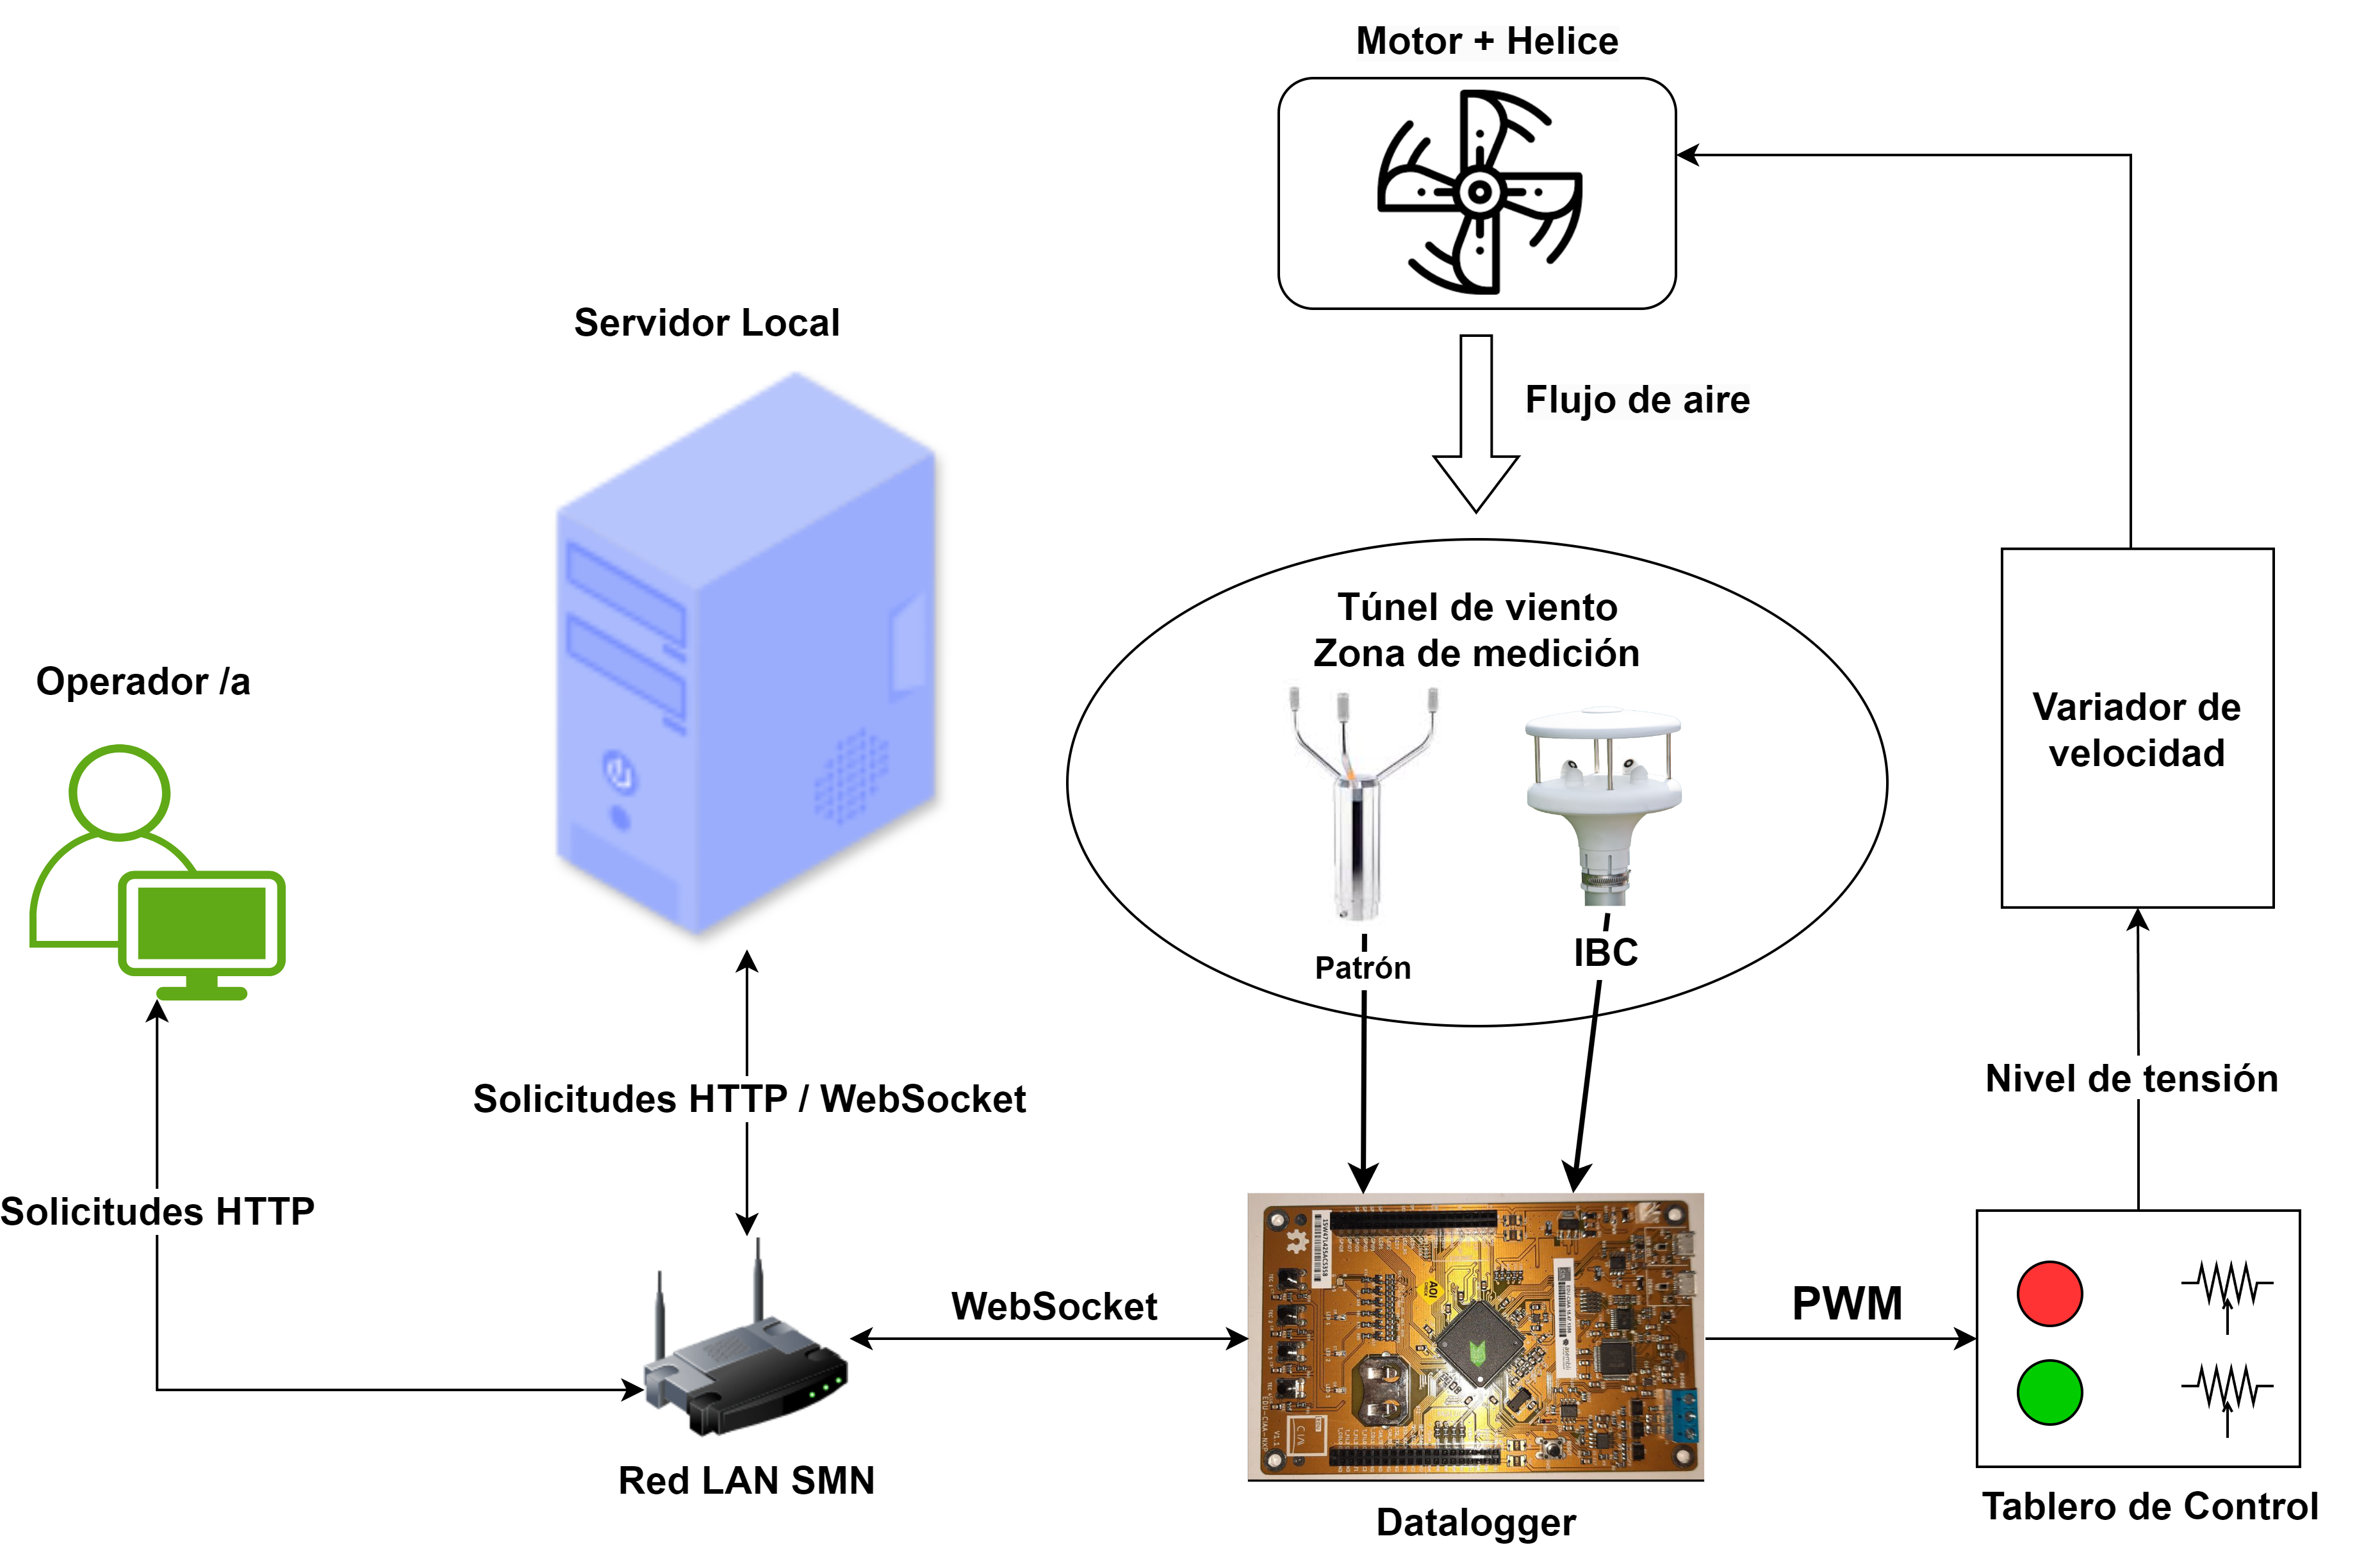
\includegraphics[width=1\linewidth]{Figuras/introduccion/sistemaDesarrollado.png}
    \caption{Sistema de calibración a desarrollar.} 
    \label{fig:sistemaDesarrollado}
\end{figure}

Dicho sistema deberá aplicar de forma automatizada los procedimientos actuales de calibración de anemómetros de ultrasonido en un túnel de viento y el mismo estará compuesto de:
\begin{enumerate}
    \item Un sistema de control basado en la placa de desarrollo EDU-CIAA, que permita la adquisición y transmisión de datos medidos por sensores de viento, hacia un servidor, mediante un enlace de comunicación Ethernet y permita automatizar el cambio de velocidades del túnel de viento, utilizando un circuito con una señal de control PWM, que reemplaza el comando manual que regula la velocidad del motor, actualmente controlada con potenciómetros.
     
    \item Una aplicación web desarrollada con el \textit{framework} Django en Python que permita:
    \begin{itemize}
        \item Configurar los sistemas de adquisición y control.
        \item Cargar los metadatos de la calibración para elaborar el presupuesto de incertidumbre.
        \item Visualizar las mediciones en tiempo real, con la posibilidad de reiniciar las mediciones en caso de falla.
        \item Una vez finalizada la adquisición de datos, procesar las muestras y calcular la corrección y su incertidumbre combinada para cada valor de velocidad de viento medido.
        \item Guardar en la base de datos PostgreSQL tanto los datos crudos como los procesados, incluyendo los gráficos, tablas y los metadatos pertinentes.
        \item Descargar los datos crudos, procesados, gráficos y toda la información necesaria para el análisis posterior y la generación del certificado de calibración.
    \end{itemize}
\end{enumerate}
